\section{Exterior Naturally Vented~ Cavity}\label{exterior-naturally-vented-cavity}

The input object ``SurfaceProperty:ExteriorNaturalVentedCavity'' allows modeling a special case for the outside boundary conditions of heat transfer surfaces with a multi-skin exterior that is opaque.~ From the thermal envelope's point of view, the presence of a vented cavity on the outside of the surface modifies the conditions experienced by the underlying heat transfer surfaces.~ This exterior cavity acts as a radiation and convection baffle situated between the exterior environment and the outside face of the underlying heat transfer surface.~ The actual outer surface is referred to as the ``baffle''.~ The modeling here assumes that the heat capacity in the outer baffle can be neglected since it is much lower than the underlying mass surface.~ This object is used with the BuildingSurface:Detailed object where the heat transfer surfaces are referred to as the underlying surfaces.~ The constructions and materials for the heat transfer surfaces should reflect the construction of just the underlying surface.~ The SurfaceProperty:ExteriorNaturalVentedCavity object is used to describe the detached layer, or baffle, and the characteristics of the cavity and openings for natural ventilation.~ This model uses the SurfaceProperty:OtherSideConditionsModel object to pass boundary conditions to the heat transfer modeling for the underlying surfaces.

\subsection{Baffle Heat Balance}\label{baffle-heat-balance}

The baffle is assumed to be sufficiently thin and high-conductivity so that it can be modeled using a single temperature (for both sides and along its area).~ This temperature \({T_{s,baff}}\) is determined by formulating a heat balance on a control volume that just encapsulates the baffle surface.~ The baffle is assumed to completely cover the underlying surface such that it is opaque to shortwave and longwave radiation.~ This assumption means that even though the baffle will have some open area for ventilation, no solar energy passes through these openings. The heat balance is diagrammed in the following figure.

\begin{figure}[hbtp] % fig 33
\centering
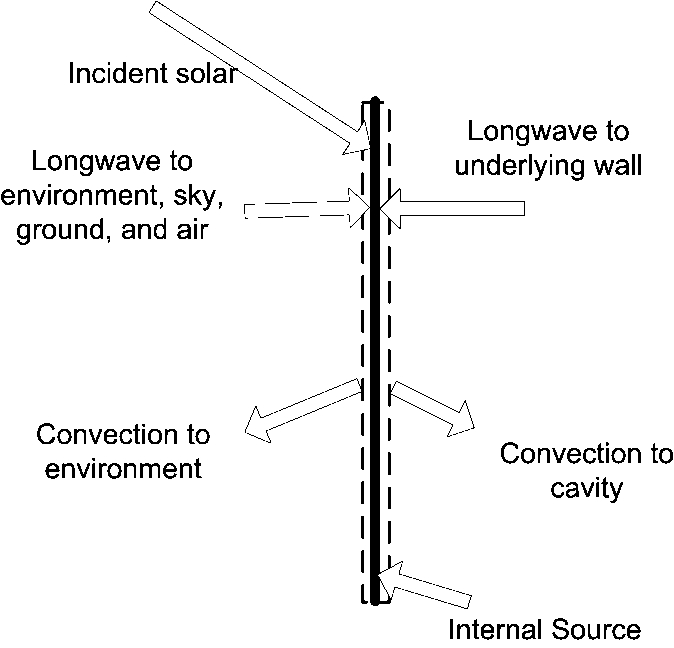
\includegraphics[width=0.9\textwidth, height=0.9\textheight, keepaspectratio=true]{media/image438.png}
\caption{Baffle Surface Heat Balance \protect \label{fig:baffle-surface-heat-balance}}
\end{figure}

The heat balance on the baffle surface's control volume is:

\begin{equation}
{q''_{\alpha sol}} + {q''_{LWR,Env}} + {q''_{conv,Env}} + {q''_{LWR,cav}} + {q''_{conv,cav}} + {q''_{source}} = 0
\end{equation}

where: 
\(q''_{\alpha sol}\) is absorbed direct and diffuse solar (short wavelength) radiation heat flux.
\(q''_{LWR,Env}\) is net long wavelength (thermal) radiation flux exchange with the air and surroundings.
\(q''_{conv,Env}\) = surface convection flux exchange with outside air.
\(q''_{LWR,cav}\) is net long wavelength (thermal) radiation flux exchange with the outside face of the underlying surface(s).
\(q''_{conv,cav}\) = surface convection flux exchange with cavity air.
\({q''_{source}}\) is a source/sink term that accounts for energy exported out of the control volume when the baffle is a hybrid device such as a photovoltaic panel.

All terms are positive for net flux to the baffle.~ Each of these heat balance components is introduced briefly below.

\subsubsection{External SW Radiation}\label{external-sw-radiation}

\(q''_{\alpha sol}\)~is calculated using procedures presented elsewhere in this manual and includes both direct and diffuse incident solar radiation absorbed by the surface face.~ This is influenced by location, surface facing angle and tilt, shading surfaces, surface face material properties, weather conditions, etc.~ The baffle blocks all shortwave radiation from reaching the underlying surface.

\subsubsection{External LW Radiation}\label{external-lw-radiation}

\({q''_{LWR,Env}}\) ~is a standard radiation exchange formulation between the surface, the sky, the ground, and the atmosphere.~ The radiation heat flux is calculated from the surface absorptivity, surface temperature, sky, air, and ground temperatures, and sky and ground view factors.~ Radiation is modeled using linearized coefficients. ~The baffle blocks all longwave radiation.

\subsubsection{External Convection}\label{external-convection}

\(q''_{conv,env}\) is modeled using the classical formulation: \(q''_{conv} = h_{co}(T_{air} - T_{o})\) where h\(_{co}\), is the convection coefficient.~ The h\(_{co}\) is treated in the same way as an outside face with ExteriorEnvironment conditions.~ In addition, when it is raining outside, we assume the baffle gets wet and model the enhanced surface heat transfer using a large value for \({h_{co}}\) .

\subsubsection{Cavity LW Radiation}\label{cavity-lw-radiation}

\({q''_{LWR,cav}}\) is a standard radiation exchange formulation between the baffle surface and the underlying heat transfer surface located across the cavity.~ Radiation is modeled using linearized coefficients.

\subsubsection{Cavity Convection}\label{cavity-convection}

\(q''_{conv,cav}\) is modeled using the classical formulation: \(q''_{conv} = h_{cp}(T_{air} - T_{o})\) where h\(_{cp}\), is the convection coefficient. The value for h\(_{cp}\) is obtained from correlations used for window gaps from ISO (2003) standard 15099.

Substituting models into (113) and solving for \({T_{s,baff}}\) ~yields the following equation:

\begin{equation}
{T_{s,baff}} = \frac{{\left( {{I_s}\alpha  + {h_{co}}{T_{amb}} + {h_{r,atm}}{T_{amb}} + {h_{r,sky}}{T_{sky}} + {h_{r,gnd}}{T_{amb}} + {h_{r,cav}}{T_{so}} + {h_{c,cav}}{T_{a,cav}} + {{q''}_{source}}} \right)}}{{\left( {{h_{co}} + {h_{r,air}} + {h_{r,sky}} + {h_{r,gnd}} + {h_{r,cav}} + {h_{c,cav}}} \right)}}
\end{equation}

where,

\({I_s}\) ~is the incident solar radiation of all types {[}W/m\(^{2}\){]},

\(\alpha\) ~is the solar absorptivity of the baffle {[}dimensionless{]},

\({h_{r,atm}}\) is the linearized radiation coefficient for the surrounding atmosphere {[}W/m\(^{2}\)·K{]},

\({T_{amb}}\) ~is the outdoor drybulb from the weather data, also assumed for ground surface {[}ºC{]},

\({h_{r,sky}}\) ~is the linearized radiation coefficient for the sky {[}W/m\(^{2}\)·K{]},

\({T_{sky}}\) ~is the effective sky temperature {[}ºC{]},

\({h_{r,gnd}}\) ~is the linearized radiation coefficient for the ground {[}W/m\(^{2}\)·K{]},

\({h_{r,cav}}\) ~is the linearized radiation coefficient for the underlying surface {[}W/m\(^{2}\)·K{]},

\({T_{so}}\) ~is the temperature of the outside face of the underlying heat transfer surface {[}ºC{]},

\({h_{co}}\) ~is the convection coefficient for the outdoor environment {[}W/m\(^{2}\)·K{]},

\({h_{c,cav}}\) ~is the convection coefficient for the surfaces facing the plenum {[}W/m\(^{2}\)·K{]}, and

\({T_{a,cav}}\) ~is the drybulb temperature for air in the cavity {[}ºC{]}.

\subsection{Cavity Heat Balance}\label{cavity-heat-balance}

The \emph{cavity} is the volume of air located between the baffle and the underlying heat transfer surface.~ The cavity air is modeled as well-mixed.~ The uniform temperature of the cavity air, \({T_{a,cav}}\) , is determined by formulating a heat balance on a control volume of air as diagrammed below.

\begin{figure}[hbtp] % fig 34
\centering
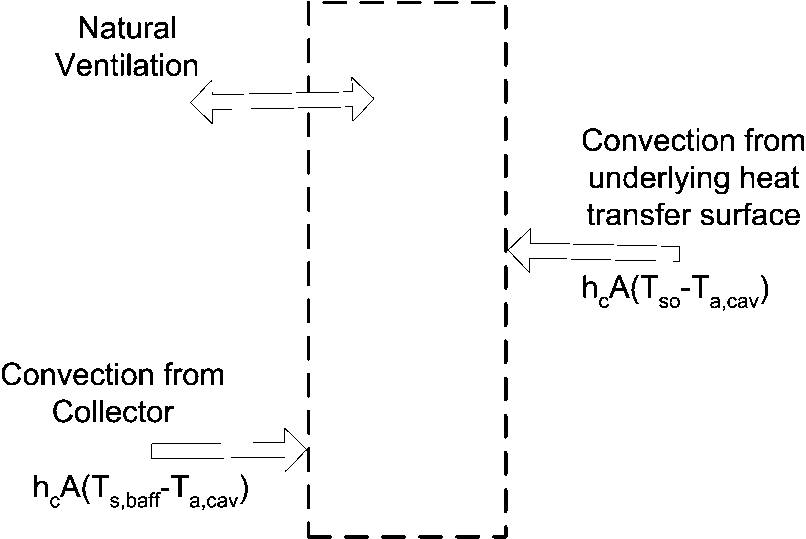
\includegraphics[width=0.9\textwidth, height=0.9\textheight, keepaspectratio=true]{media/image469.png}
\caption{Cavity Air Heat Balance \protect \label{fig:cavity-air-heat-balance}}
\end{figure}

The heat balance on the cavity air control volume is:

\begin{equation}
{\dot Q_{vent}} + {\dot Q_{co}} + {\dot Q_{c,baff}} = 0
\end{equation}

where,

\(\dot{Q}_{vent}\) is the net rate of energy added from natural ventilation -- where outdoor ambient air exchanges with the cavity air. \(\dot{Q}_{co}\) is the net rate of energy added by surface convection heat transfer with the underlying surface.

\({\dot Q_{c,baff}}\) is the net rate of energy added by surface convection heat transfer with the collector.

And substituting into yields the following equation:

\begin{equation}
{T_{a,cav}} = \frac{{\left( {{h_{c,cav}}A\,{T_{so}} + {{\dot m}_{vent}}{c_p}{T_{amb}} + {h_{c,cav}}A\,{T_{s,baff}}} \right)}}{{\left( {{h_{c,cav}}A + {{\dot m}_{vent}}{c_p} + {h_{c,cav}}A} \right)}}
\end{equation}

where,

\({\dot m_{vent}}\) ~is the air mass flow from natural forces {[}kg/s{]}

Modeling natural ventilation air exchanges in a general way is challenging.~ Simplistic engineering models are used to model \({\dot m_{vent}}\) ~resulting from natural buoyancy and wind forces.~ Reasoning that the configuration is similar to single-side natural ventilation, we elect to use correlations for natural ventilation presented as equations (29) and (30) in Chapter 26. of ASHRAE HOF (2001).

\begin{equation}
{\dot m_{vent}} = \rho \,{{\rm{\rlap{--} \dot V}}_{{\rm{tot}}}}
\end{equation}

where,

\(\rho\) ~is the density of air {[}kg/m\(^{3}\){]}, and

\(\rlap{--} \dot{V}_{tot} = \rlap{--} \dot{V}_{wind} + \rlap{--} \dot{V}_{thermal}\) ~is the total volumetric flow rate of air ventilating in and out of the cavity.

\begin{equation}
\rlap{--} \dot{V}_{wind} = C_{v}A_{in}U_{\infty}
\end{equation}

\begin{equation}
\rlap{--} \dot{V}_{thermal} = \left\{
    \begin{array}{cl}
      C_{D}A_{in}\sqrt{2g\Delta H_{NPL}\left(T_{a,cav}-T_{amb}\right)/T_{a,cov}} & \; \left(T_{a,cav} > T_{amb}\right) \\
      C_{D}A_{in}\sqrt{2g\Delta H_{NPL}\left(T_{amb}-T_{a,cav}\right)/T_{amb}} & \; \left(T_{a,cav} < T_{amb}\,\text{and baffle is vertical}\right) 
    \end{array}
  \right.
\end{equation}

\({{\rm{\rlap{--} \dot V}}_{{\rm{thermal}}}} = {C_D}{A_{in}}\sqrt {2g\Delta {H_{NPL}}\left( {{T_{a,cav}} - {T_{amb}}} \right)/{T_{a,cav}}}\) ~ (if \(T_{a,cav} > T_{amb}\) )

\({{\rm{\rlap{--} \dot V}}_{{\rm{thermal}}}} = {C_D}{A_{in}}\sqrt {2g\Delta {H_{NPL}}\left( {{T_{amb}} - {T_{a,cav}}} \right)/{T_{amb}}}\) ~ (if \(T_{amb} > T_{a,cav}\) ~and baffle is vertical)

\({C_v}\) ~is the effectiveness of the openings that depends on opening geometry and the orientation with respect to the wind.~ ASHRAE HoF (2001) indicates values ranging from 0.25 to 0.6.~ This value is available for user input.

\({C_D}\) ~is the discharge coefficient for the opening and depends on opening geometry.~ This value is available for user input.

Mass continuity arguments lead to modeling the area of the openings as one half of the total area of the openings, so we have:

\begin{equation}
{A_{in}} = \frac{{A\,}}{2}
\end{equation}

\(g\) ~is the gravitational constant taken as 9.81 {[}m/s\(^{2}\){]}.

\(\Delta {H_{NPL}}\) ~is the height from midpoint of lower opening to the Neutral Pressure Level.~ This is value is available for user input.

If the cavity is horizontal and \(T_{amb} > T_{a,cav}\) ~then \({{\rm{\rlap{--} \dot V}}_{{\rm{thermal}}}}{\rm{ = 0}}\) ~because this is a stable situation.

\subsection{Underlying Heat Transfer Surface}\label{underlying-heat-transfer-surface}

The exterior baffle and cavity are applied to the outside of a heat transfer surface.~ This surface is modeled using the usual EnergyPlus methods for handling heat capacity and transients -- typically the CTF method.~ These native EnergyPlus heat balance routines are used to calculate \({T_{so}}\) .~ The exterior baffle and cavity system is coupled to the underlying surface using the SurfaceProperty:OtherSideConditionsModel mechanism.~ The exterior naturally vented cavity model provides values for \({h_{r,cav}}\) ,\({T_{s,baff}}\) , \({h_{c,cav}}\) , and \({T_{a,cav}}\) ~for use with the heat balance model calculations for the outside face of the underlying surface (described elsewhere in this manual).

\subsection{Solar and Shading Calculations}\label{solar-and-shading-calculations}

The exterior vented cavity model uses standard EnergyPlus surfaces in order to take advantage of the detailed solar and shading calculations.~ Solar radiation incident on the surface includes beam and diffuse radiation, as well as radiation reflected from the ground and adjacent surfaces.~ Shading of the collector by other surfaces, such as nearby buildings or trees, is also taken into account.

\subsection{Local Wind Speed Calculations}\label{local-wind-speed-calculations}

The outdoor wind speed affects terms used in modeling.~ The wind speed in the weather file is assumed to be measured at a meteorological station located in an open field at a height of 10 m.~ To adjust for different terrain at the building site and differences in the height of building surfaces, the local wind speed is calculated for each surface.

The wind speed is modified from the measured meteorological wind speed by the equation (ASHRAE 2001):

\begin{equation}
{U_\infty } = {V_{met}}{\left( {\frac{{{\delta_{met}}}}{{{z_{met}}}}} \right)^{{a_{met}}}}{\left( {\frac{z}{\delta }} \right)^a}
\end{equation}

where z is the height of the centroid of the system, z\(_{met}\) is the height of the standard meteorological wind speed measurement, and a and d are terrain-dependent coefficients.~ d is the boundary layer thickness for the given terrain type.~ The values of a and d are shown in the following tables:

% table 19
\begin{longtable}[c]{@{}llll@{}}
\caption{Terrain-Dependent Coefficients (ASHRAE 2001). \label{table:terrain-dependent-coefficients-ashrae-2001.}} \tabularnewline
\toprule 
Terrain & Description & Exponent, a & Layer Thickness, $\delta$ (m) \tabularnewline
\midrule
\endfirsthead

\caption[]{Terrain-Dependent Coefficients (ASHRAE 2001).} \tabularnewline
\toprule 
Terrain & Description & Exponent, a & Layer Thickness, $\delta$ (m) \tabularnewline
\midrule
\endhead

1 & Flat, open country & 0.14 & 270 \tabularnewline
2 & Rough, wooded country & 0.22 & 370 \tabularnewline
3 & Towns and cities & 0.33 & 460 \tabularnewline
4 & Ocean & 0.10 & 210 \tabularnewline
5 & Urban, industrial, forest & 0.22 & 370 \tabularnewline
\bottomrule
\end{longtable}

The exterior vented cavity can be defined such that it has multiple underlying heat transfer surfaces.~ The centroid heights for each surface are area-weighted to determine the average height for use in the local wind calculation.

\subsection{Convection Coefficients}\label{convection-coefficients}

Exterior cavity modeling requires calculating up to three different coefficients for surface convection heat transfer.~ These coefficients are defined in the classic way by:

\begin{equation}
{h_c} = \frac{{{T_{air}} - {T_{surf}}}}{{{{q''}_{conv}}}}
\end{equation}

First, \({h_{co}}\) ~is the convection coefficient for the baffle surface facing the outdoors.~ It is modeled in exactly the same way as elsewhere in EnergyPlus and will depend on the user setting for Outside Convection Algorithm -- Outside Surface Heat Balance entry elsewhere in this document.

Second, \({h_{c,cav}}\) ~is the convection coefficient for baffle surfaces facing the cavity.~ This coefficient is applied to both the baffle and the underlying surface.~ The convection coefficient is modeled in the same way used in EnergyPlus to model air gaps in windows.~ These correlations vary by Rayleigh number and surface tilt and are based on the work of various research including Hollands et. al., Elsherbiny et. al., Wright, and Arnold.~ The formulations are documented in ISO (2003) standard 15099.~ The routines were adapted from Subroutine NusseltNumber in WindowManager.f90 (by F. Winkelmann), which itself was derived from Window5 subroutine ``nusselt''.

\subsection{Radiation Coefficients}\label{radiation-coefficients}

Exterior vented cavity modeling requires calculating up to four different linearized coefficients for radiation heat transfer.~ Whereas radiation calculations usually use temperature raised to the fourth power, this greatly complicates solving heat balance equations for a single temperature.~ Linearized radiation coefficients have the same units and are used in the same manner as surface convection coefficients and introduce very little error for the temperature levels involved.

The radiation coefficient, \({h_{r,cav}}\) , is used to model thermal radiation between the collector surface and the outside face of the underlying heat transfer surface.~ We assume a view factor of unity.~ It is calculated using:

\begin{equation}
{h_{r,cav}} = {\sigma_{SB}}{e_{baff}}{e_{so}}\frac{{\left( {T_{s,baff}^4 - T_{so}^4} \right)}}{{\left( {{T_{s,baff}} - {T_{so}}} \right)}}
\end{equation}

where,

all temperatures are converted to Kelvin,

\({\sigma_{SB}}\) ~is the Stefan-Boltzmann constant,

\({e_{baff}}\) ~is the longwave thermal emittance of the baffle, and

\({e_{so}}\) ~is the longwave thermal emittance of the underlying heat transfer surface.

The three other coefficients, \({h_{r,atm}}\) , \({h_{r,sky}}\) , and \({h_{r,gnd}}\) ~are used elsewhere in EnergyPlus for the outside face surface heat balance and are calculated in the same manner as equation .~ {[}This is accomplished by calling subroutine InitExteriorConvectionCoeffs in the file HeatBalanceConvectionCoeffs.f90. {]}

\subsection{References}\label{references-023}

ASHRAE HOF 2001.~ 2001 ASHRAE Fundamentals Handbook.~ American Society of Heating Refrigeration and Air-Conditioning Engineers. Altanta GA.

ISO. 2003. ISO 15099:2003. Thermal performance of windows, doors, and shading devices -- Detailed calculations. International Organization for Standardization.
